\documentclass[a4paper,11pt]{article}
\usepackage{graphicx}
\usepackage{enumerate}
\usepackage[usenames, dvipsnames]{color}

\begin{document}

\begin{flushright}

\vspace{1.1cm}

{\bf\Huge Problem Set 7}

\rule{0.25\linewidth}{0.5pt}

\vspace{0.5cm}
%Put Authors
Justin Ely
\linebreak
\newline
%Put Author's affiliations
\footnotesize{605.411 Foundations of Computer Architecture \\}
\vspace{0.5cm}
% Date here below
31 October, 2016
\end{flushright}

\noindent\rule{\linewidth}{1.0pt}

%%%%%%%%%%%%%%%%%%%%%%%%%%%%%%%%%%%%%%%%%%%%%%%%%%%%%%%%%%

\section*{1a)}
With branch outcomes determined in the EX stage, each mis-prediction
will need three NOPs to clear the pipeline, and thus will cause three missed
cycles in 55\% (100-45\%) of the BEQ instructions.  Thus the extra CPI is $3 \times .55 \times .25 = .4125$.

\section*{1b)}
The two bit predictor is only incorrect 15\% of the time, thus the extra CPI is 
$3 \times .15 \times .25 = .1125$.

\section*{1c)}
If the branch instructions could be replaced by ALU instructions, there would
be no miss-predicted branches.  Thus the extra cycles would be 0.  Speedup would
then be $\frac{1.1125}{1.0} = 1.1125$.

%%%%%%%%%%%%%%%%%%%%%%%%%%%%%%%%%%%%%%%%%%%%%%%%%%%%%%%%%%

\section*{2a)} 
Branch prediction addresses control hazards by attempting to reduce stalls
by guessing the likely outcome of a branch. If no guessing was made, stalls 
would be necessary.  With accurate prediction, guessing is correct more often 
than wrong and results in fewer wasted cycles.

\section*{2b)}
Instruction scheduling addresses both structural and data hazards.  
This technique re-arranges instructions with dependencies so that, as much 
as possible, no delays need to be introduced.


\section*{2c)}
Delay slots address data hazards by inserting instructions with no dependence
on a load-instruction into the cycle immediately following.  This makes sure
that any instruction requiring the output of the load is sufficiently separated
to avoid needing a stall.


\section*{2d)}
Increased availability of functional units addresses structural hazards by 
making sure that any given instruction is not monopolizing hardware necessary
for another pipelined instruction.

%%%%%%%%%%%%%%%%%%%%%%%%%%%%%%%%%%%%%%%%%%%%%%%%%%%%%%%%%%

\section*{3a)}
\begin{tabular}{| c | c |}
  \hline	
  	Prediction & Outcome \\ \hline \hline
	NT & T \\ \hline
	NT & NT \\ \hline
	NT & T \\ \hline
	NT & T \\ \hline
	T & NT \\ \hline
\end{tabular} \\

The two-bit predictor is only correct $\frac{1}{5}$ of the time for an accuracy of 20\%.

\section*{3b)}
Coding the predictor in python, and running through a sequence of 50,000 
branches hit 0.59992\%.  Presumably this limit hits 60\% for infinite trials.


\section*{3c)}
The perfect predictor would be exactly the same as the pattern: T $->$ NT $->$ T $->$ T $->$ NT $->$ (start).  Any mis-prediction would also return to start.
Thus, at most a handful of mispredictions would happen before the predictor aligned with the pattern.

\section*{3d)}
{\bf Presuming the question meant c, not d:} \\

\begin{tabular}{| c | c |}
  \hline	
  	Prediction & Outcome \\ \hline \hline
	T & NT \\ \hline
	T & T \\ \hline
	NT & NT \\ \hline
	T & NT \\ \hline
	T & T \\ \hline
\end{tabular} \\

This predictor would hit $\frac{3}{5}$ or 60\% for one pass through the pattern.

%%%%%%%%%%%%%%%%%%%%%%%%%%%%%%%%%%%%%%%%%%%%%%%%%%%%%%%%%%

\section*{4a)}

\begin{figure}[h!]
\caption{Program execution} 
\centering
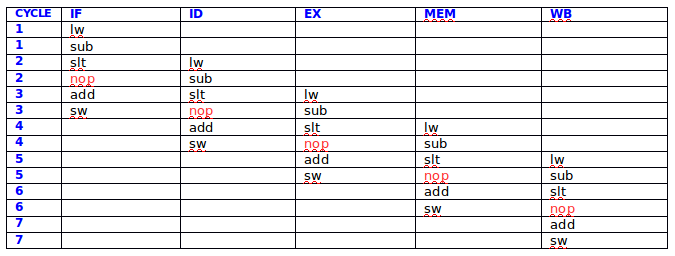
\includegraphics[width=1.1\textwidth]{hw7_p4a.png}
\end{figure}

\section*{4b)}
\begin{itemize}
  \item In cycle 1, the lw and add instructions will be fetched.  
  \item In cycle 2, lw and add 
will be send to the reservation station, sub and slt will be fetched.  
  \item In cycle 3, lw will be sent to the load/store functional unit for execution.  
Also, sub and slt will be sent to the reservation station and sw will be fetched.
  \item In cycle 4, lw will be send to the memory stage, sub and slt will be sent to the
integer functional units for execution, and sw will be sent to the reservation
station.  
  \item In cycle 5, lw will be sent to the wb stage, add will move to the 
integer functional unit for execution, sub and slt will be sent to the wb stage, and sw will be send to the load/store functional unit for execution.
  \item In cycle 6, add will be sent to the wb stage, and sw will be sent to the memory
stage.
\end{itemize}

%%%%%%%%%%%%%%%%%%%%%%%%%%%%%%%%%%%%%%%%%%%%%%%%%%%%%%%%%%


\end{document}
